\documentclass[conference]{IEEEtran}

  \usepackage{booktabs}
  \usepackage{listing}
  \usepackage{amsmath}
  \usepackage{algorithm}
  \usepackage{array}
  \usepackage{url}
  \usepackage{cite}
  \usepackage{complexity}
  \usepackage{algpseudocode}
   \usepackage{graphicx}
   \usepackage{enumerate}
   \usepackage{subcaption}
   \usepackage[shortlabels]{enumitem}


% \usepackage{algorithm}
  \ifCLASSINFOpdf
  
  \else
  
  \fi
  
  \hyphenation{op-tical net-works semi-conduc-tor}
  
  \begin{document}
  
  \title{Evolutionary Neural Architecture Search for Image Classifier \\ Mid-term Report}
  
  \author{\IEEEauthorblockN{Bowen Zheng, Shijie Chen, Shuxin Wang}
  \IEEEauthorblockA{Department of Computer Science and Engineering\\
  Southern University of Science and Technology\\
  Shenzhen, Guangdong, China\\}
  }
  
  \maketitle
  
  \begin{abstract}
  EvoNAS project
  \end{abstract}
  \IEEEpeerreviewmaketitle
  
  \section{Introduction}
  

  \section{Proposed Framework}
 
  \begin{table}[H]
    
    \centering
      \begin{tabular}{cccc}
      \toprule
      Variable&Name\\
      \midrule
     
      $N_{total}$&size of the total population\\
  \bottomrule
  \end{tabular}
  \caption{Notation}
  \label{table:1}
  \end{table}

  \subsection{Fuzzy Rules}
  
  \begin{figure}[H]
 	\centering
 	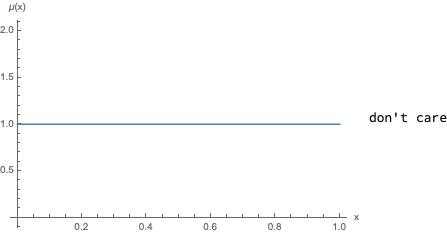
\includegraphics[width=0.4\textwidth]{figures/u1.png}
   \caption{The $don't care$ function}\label{fig:digit}
   \label{u0}
 \end{figure}
 \begin{figure}[H]
 	\centering
 	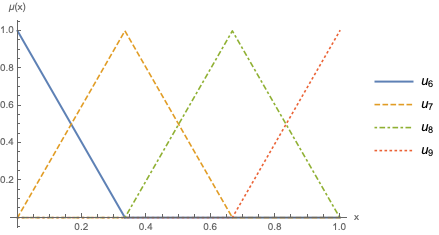
\includegraphics[width=0.4\textwidth]{figures/u4.png}
   \caption{Membership Functions with 4 intervals}\label{fig:digit}
   \label{u3}
 \end{figure}
  The antecedent part of $R_q$ is a set of antecedent fuzzy sets:
\begin{equation}A_q = \{A_{qi}|i = 1,2,...,n\}\end{equation}

 
  \subsection{Fuzzy Classifier}
  
  \subsection{Generate Fuzzy Rule From Training Patterns}
  
  \section{Hybrid Genetics-based Machine Learning Framework}
 
	 \subsection{NSGA-II}
	 
	 \subsubsection{Elite-preserving}
	 
	 \subsubsection{Pareto ranking}
	 
	 \subsubsection{Crowding measure}
	 
	 \subsection{Michigan-style GBML}
	 
  
   
  \section{Asynchronous Parallel Distributed System Design}
  
  \begin{figure}[H]
    \centering
    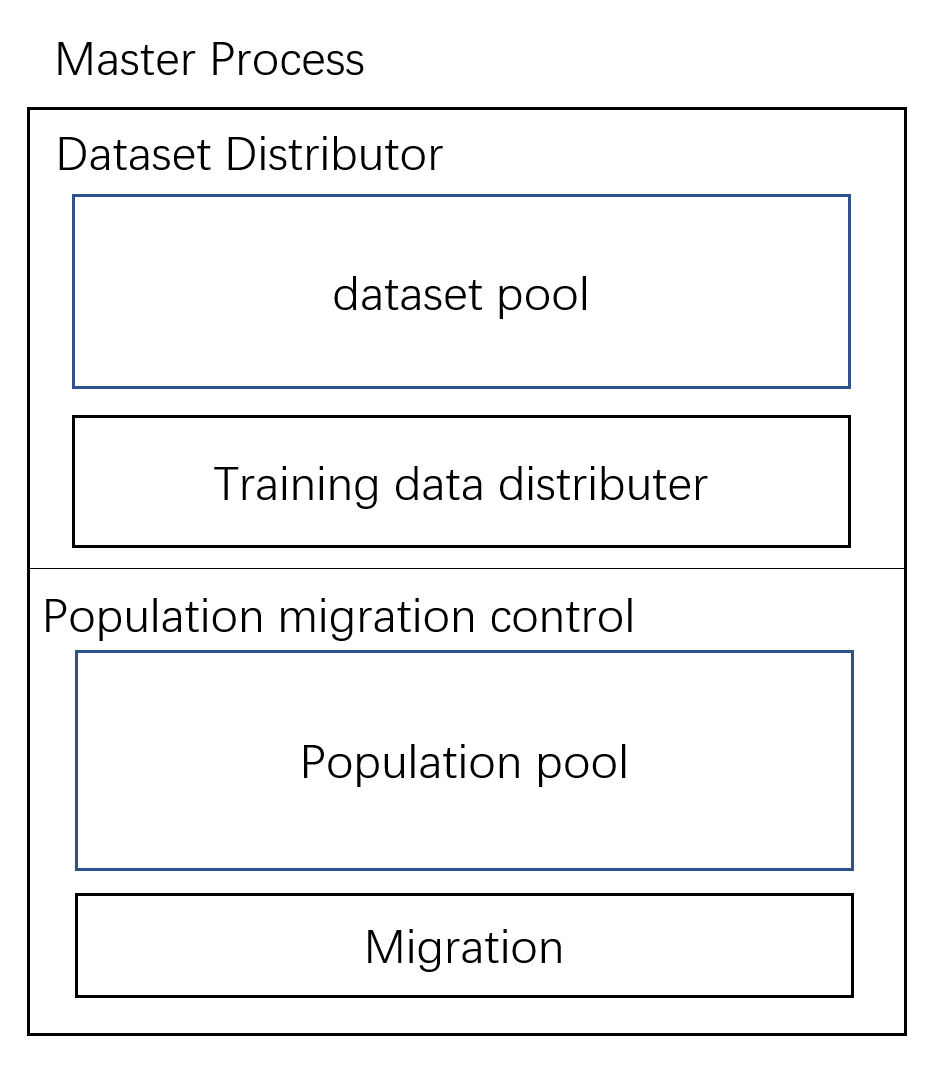
\includegraphics[width = 0.4\textwidth]{figures/master.png}
    \caption{The master process}
    \label{fig:master}
  \end{figure}

  \begin{figure}[H]
    \centering
    \includegraphics[width = 0.4\textwidth]{figures/slave.png}
    \caption{The slave process}
    \label{fig:slave}
  \end{figure}
  
  \subsection{Master and Slave process}
  \subsubsection{Master Process}
  
  \subsubsection{Slave Processes}\mbox{}
  
	\subsection{Dataset Distributor:}
	
  \subsection{Population Migration Control:}
  
	
  \subsection{Asynchronous Population Migration}
  
  
  \section{Computational Experiments}

  \subsection{Pareto Front}
  \subsubsection{With different cores}
As is shown by Fig.\ref{diffCoreTr} and Fig.\ref{diffCoreT} ($I_{update} = 100, N_{total} = 264$), our model is able to get results that is similar to non-parallel models. Note that with the increase of the number of cores, the ability of the model to obtain classifiers with more rules and antecedent fuzzy sets is decreasing, due to the decrease of sub-population. It's acceptable since our objective is to minimize the two objectives.
  \begin{figure}[H]
    \centering
    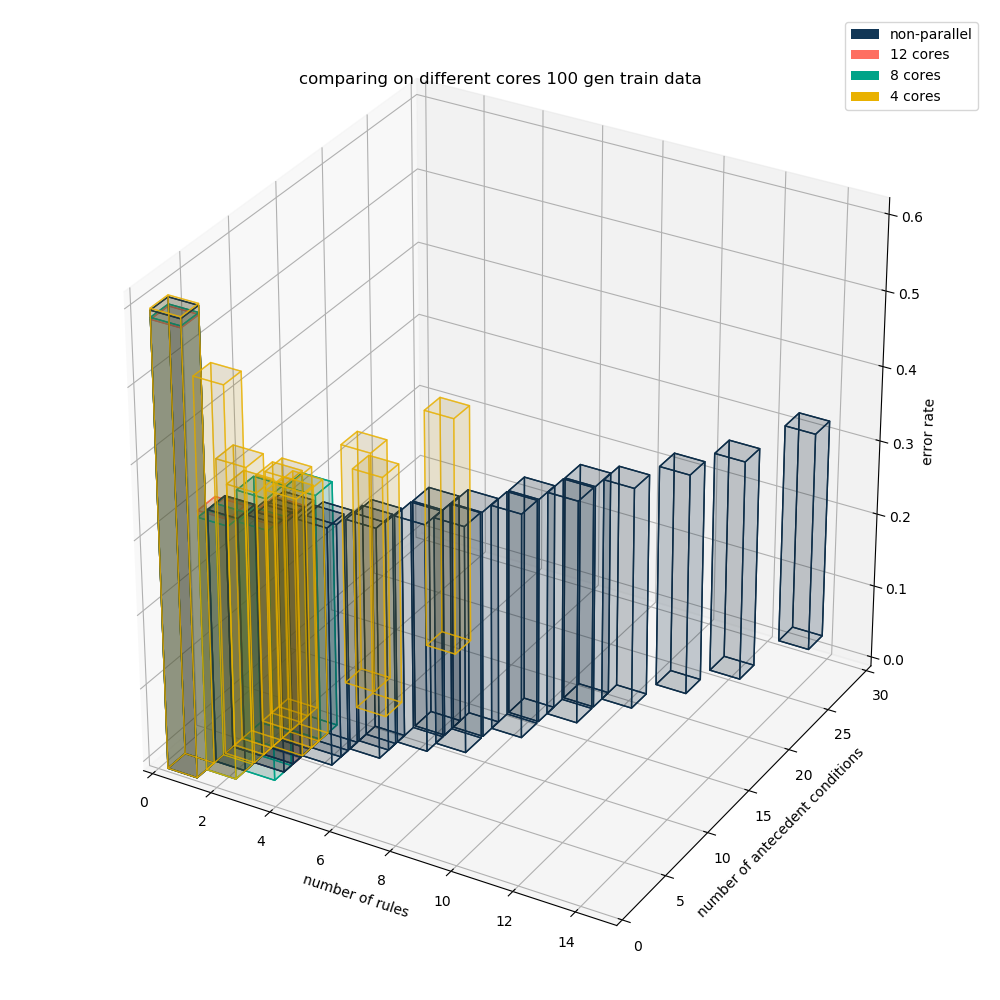
\includegraphics[width=0.38\textwidth]{figures/diffCoreTrain.png}
    \caption{Pareto Front on training data}\label{diffCoreTr}
  \end{figure}
  \begin{figure}[H]
    \centering
    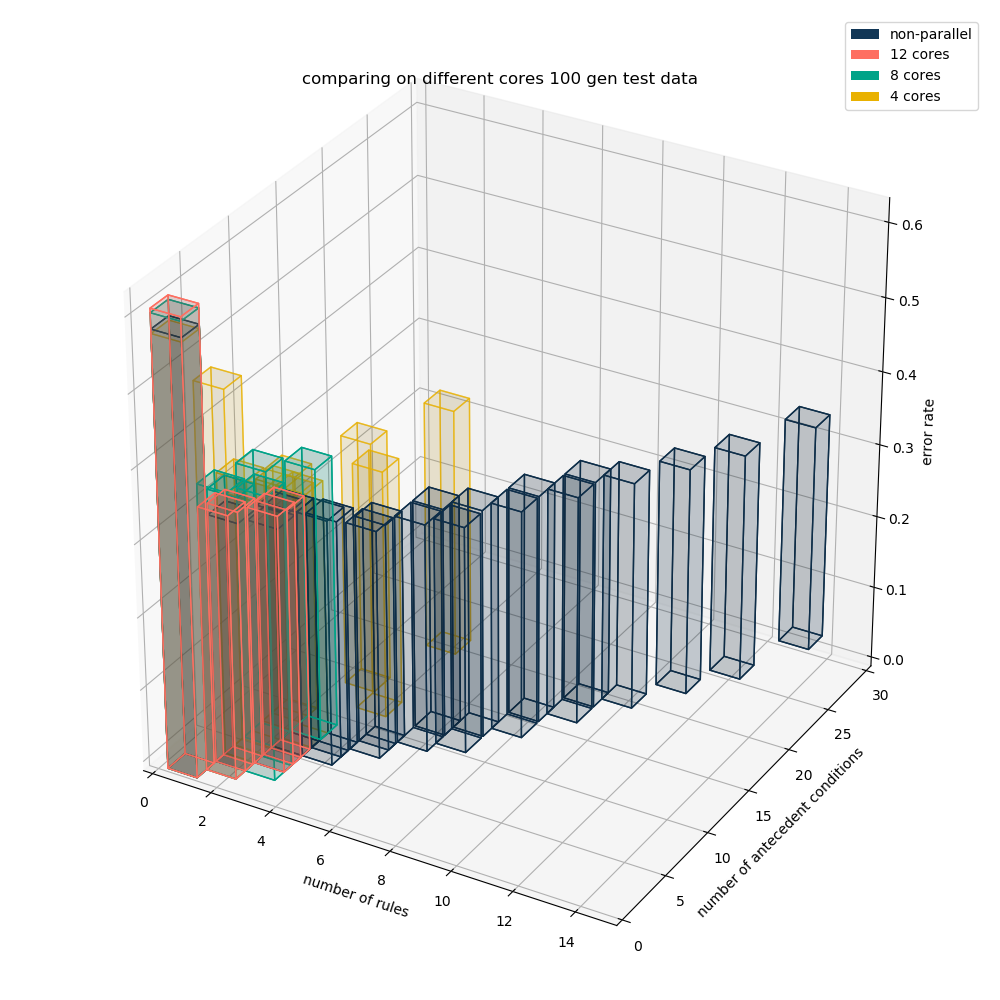
\includegraphics[width=0.38\textwidth]{figures/diffCoreTest.png}
    \caption{Pareto Front on test data}\label{diffCoreT}
  \end{figure}
  
  
  
  \subsubsection{With different exchange interval}
  We can see from Fig.\ref{diffGenTr}, Fig.\ref{diffGenT} and Fig.\ref{diffTimeGen} ($N_{total} = 264, N_{island} = 8$) that the choice of exchange interval also impacts the performance of our model. A longer exchange interval leads to less communication between master and slave processes, thus reduces running time. 
  \begin{figure}[H]
    \centering
    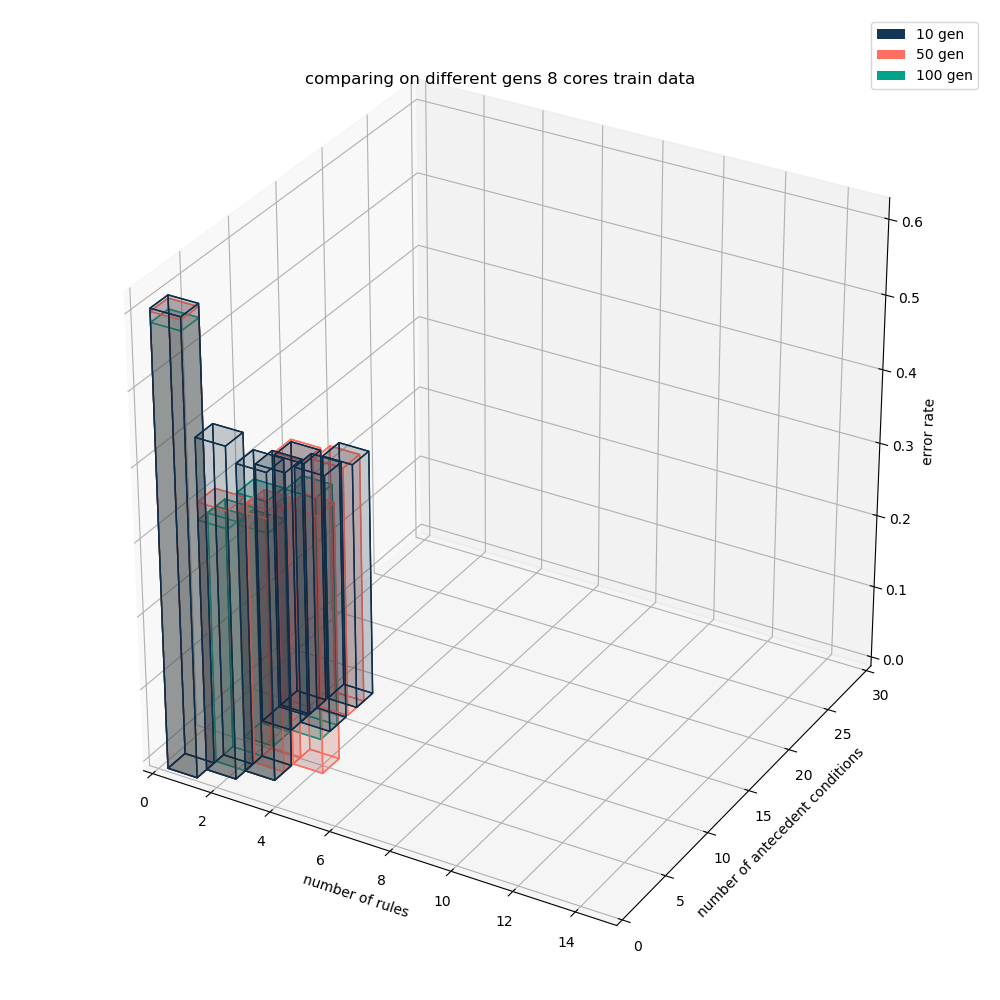
\includegraphics[width=0.4\textwidth]{figures/diffGenTrain.png}
    \caption{Pareto Front on training data with different $I_{update}$}\label{diffGenTr}
  \end{figure}
  \begin{figure}[H]
    \centering
    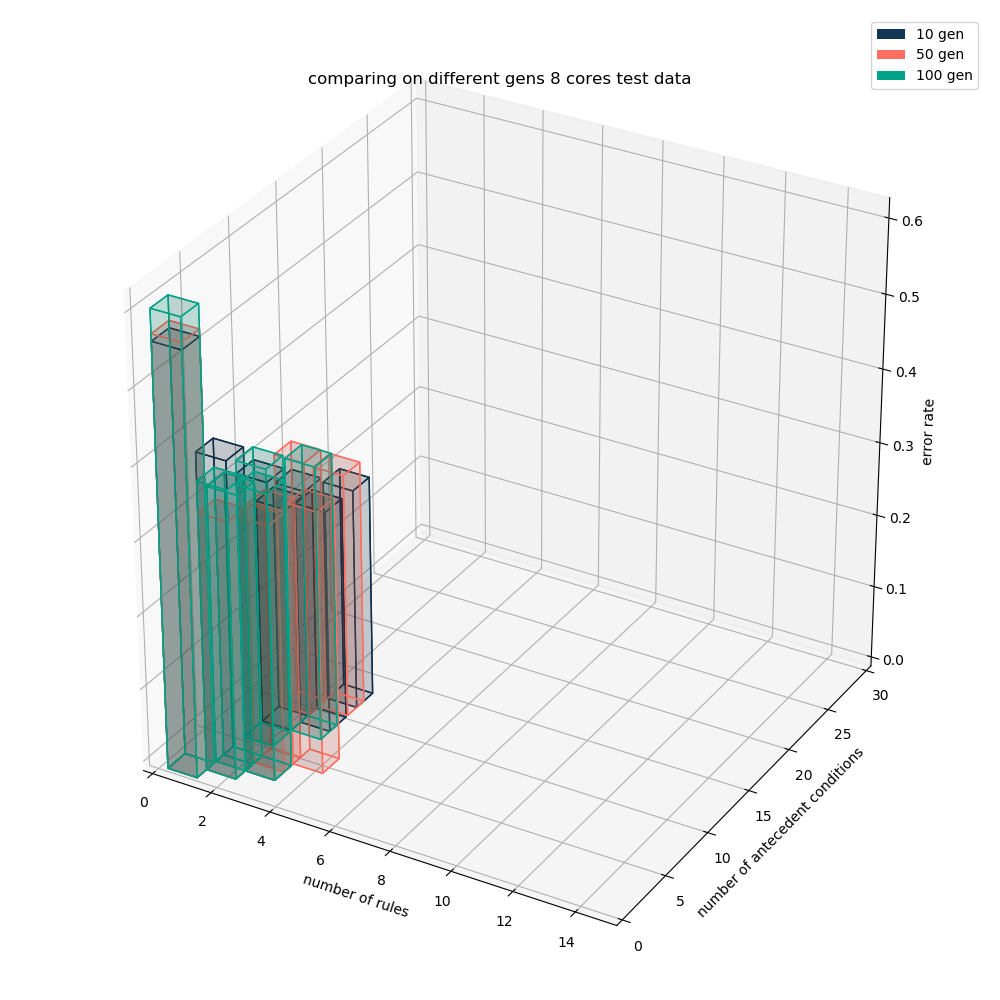
\includegraphics[width=0.4\textwidth]{figures/diffGenTest.png}
    \caption{Pareto Front on training data with different $I_{update}$}\label{diffGenT}
  \end{figure}

  \begin{figure}[H]
    \centering
    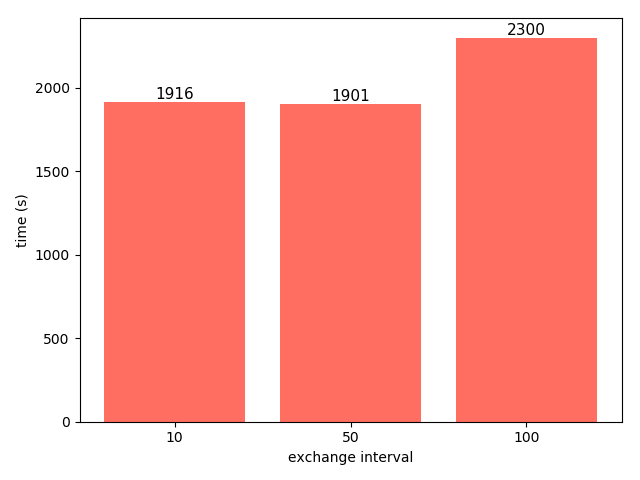
\includegraphics[width=0.4\textwidth]{figures/diffTimeGen.png}
    \caption{Computational time with different $I_{update}$}\label{diffTimeGen}
  \end{figure}



\subsection{Computation Time}
\begin{figure}[H]
  \centering
  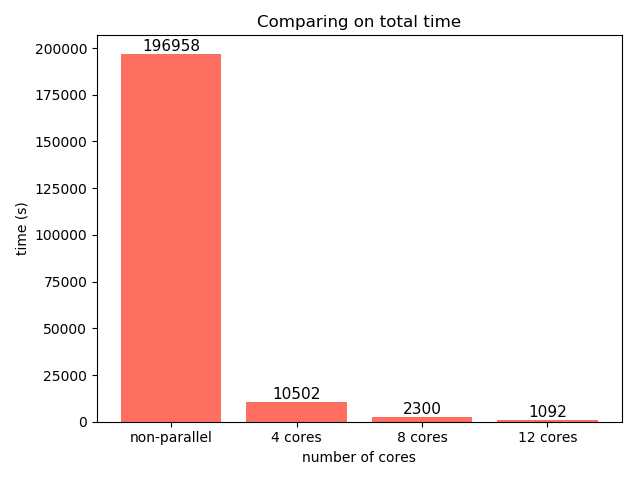
\includegraphics[width=0.4\textwidth]{figures/diffTime.png}
  \caption{Computation time of 3000 generations, $N_{pop}$ = 264.}\label{phT}
\end{figure}
With $n$ cores, we observe a speed up of up to $n^2$ times in our computational experiments.

\subsection{Compare with other model}
We compared our model with the synchronized model by Nojima et al.\cite{nojima2015application}, as is shown in Fig.\ref{diffModelTr}, Fig.\ref{diffModelTest} and Fig.\ref{diffModelTime}. The experiments are done using 8 cores.

\begin{figure}[H]
  \centering
  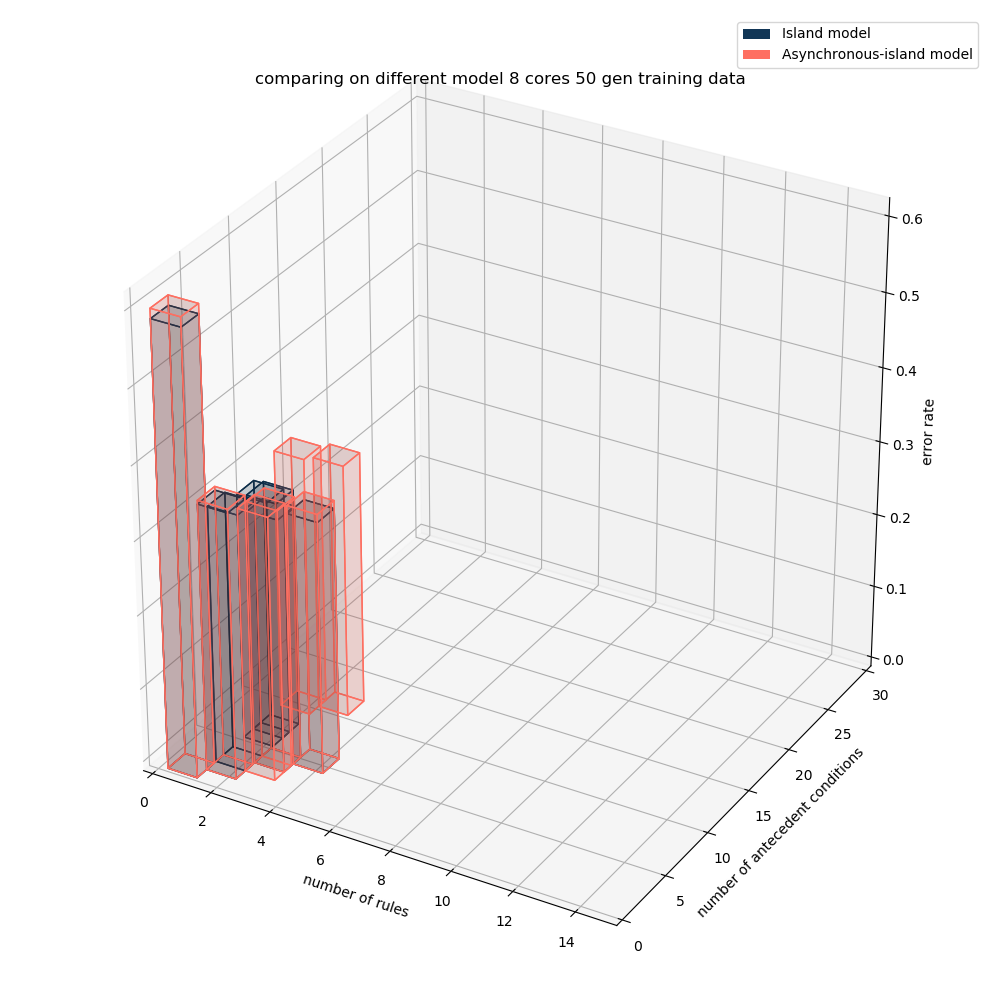
\includegraphics[width=0.4\textwidth]{figures/diffModelTrain.png}
  \caption{Comparison on training data.}\label{diffModelTr}
\end{figure}
\begin{figure}[H]
  \centering
  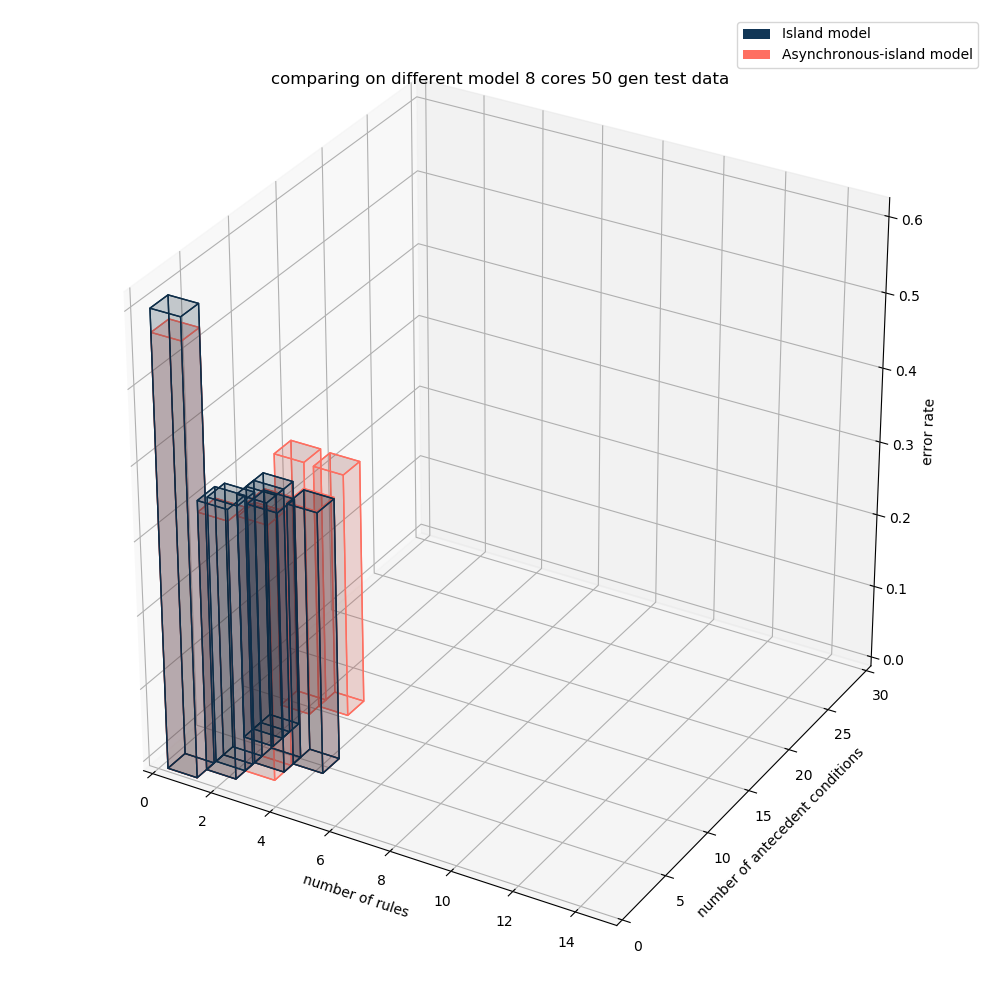
\includegraphics[width=0.4\textwidth]{figures/diffModelTest.png}
  \caption{Comparison on test data.}\label{diffModelTest}
\end{figure}
\begin{figure}[H]
  \centering
  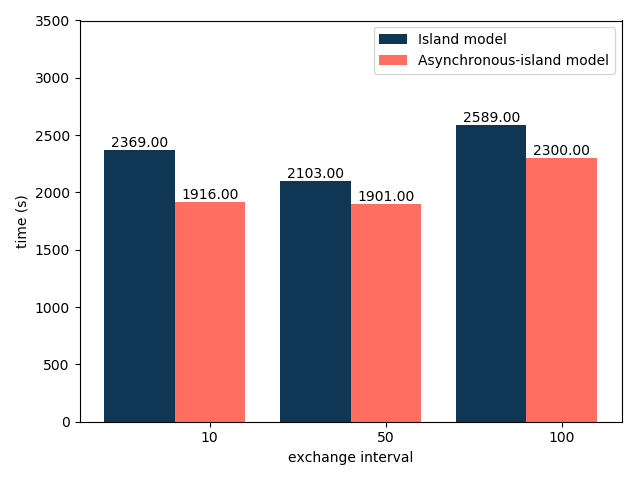
\includegraphics[width=0.4\textwidth]{figures/diffModelTime.png}
  \caption{Comparison on total time.}\label{diffModelTime}
\end{figure}


 \section{Conclusion}
 
  \section{Contribution}
  
   

\bibliographystyle{ieeetr}
\bibliography{ref}
% that's all folks
\end{document}


  